\documentclass[xcolor=table]{beamer}
\usepackage{beamerthemesplit}
\usepackage{wrapfig}
\usetheme{SPbGU}
\usepackage{pdfpages}
\usepackage{amsmath}
\usepackage{cmap}
\usepackage[T2A]{fontenc}
\usepackage[utf8]{inputenc}
\usepackage[english]{babel}
\usepackage{indentfirst}
\usepackage{amsmath}
\usepackage{tikz}
\usepackage{multirow}
\usepackage[noend]{algpseudocode}
\usepackage{algorithm}
\usepackage{algorithmicx}
\usepackage{fancyvrb}
\usetikzlibrary{shapes,arrows}
%usepackage{fancyvrb}
%\usepackage{minted}
%\usepackage{verbments}
\usepackage{fontawesome}


\beamertemplatenavigationsymbolsempty

\title[Результаты группы за 2020 год]{Результаты группы за 2020 год}
\institute[СПбГУ]{
JetBrains Research, Programming Languages and Tools Lab  \\
Санкт-Петербургский Государственный Университет
}

\author[Семён Григорьев]{Семён Григорьев}

\date{19.12.2020}

\begin{document}
{
\begin{frame}[fragile]
  \begin{tabular}{p{2.0cm} p{7.5cm} p{1cm}}
   \begin{center}
      
\includegraphics[height=1.5cm]{pictures/jetbrainsResearch.pdf}
    \end{center}
    &
    \begin{center}
      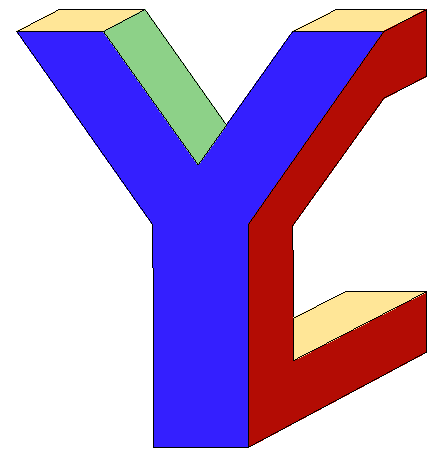
\includegraphics[height=1.5cm]{pictures/YC_logo.pdf}
    \end{center}
    &
    \begin{center}
      
\includegraphics[height=1.5cm]{pictures/SPbGU_Logo.png}
    \end{center}
  \end{tabular}
  \titlepage
\end{frame}
}


\begin{frame}[fragile]

  \frametitle{Области интересов}
\begin{itemize}
      \item Теория формальных языков
      \item Алгоритмы синтаксического анализа
      \item Применение теории формальных языков и синтаксического анализа для решения прикладных задач
      \begin{itemize}
        \item Статический анализ кода
        \item Анализ графовых баз даных
        \item Метавычисления
        \item Биоинформатика
        \item \textit{Поиск новых областей}
      \end{itemize}

\end{itemize}

\end{frame}

\begin{frame}[fragile]

  \frametitle{Состав}
\begin{itemize}
      \item Аспиранты
      \begin{itemize}
        \item Рустам Азимов
        \item Екатерина Шеметова
      \end{itemize}
      \item Магистры
      \begin{itemize}
        \item Юлия Сусанина
        \item Полина Лунина
        \item Арсений Терехов
      \end{itemize}
      \item Студенты
      \begin{itemize}
        \item Егор Орачев
        \item Влада Погожелькая
        \item Вадим Абзалов
        \item Илья Эпельбаум
        \item Тимур Зиннатулин
      \end{itemize}
      \item Работают с нами (курсовые, дипломы, семестровые проекты)
      \begin{itemize}
        \item Александра Истомина
        \item Василий Купоросов
        \item Мария Карпенко, Никита Ковалёв, Никита Влаев, Мария Назарова, Павел Алимов, \small {Дмитрий Панфилёнок, Артём Черников, \footnotesize{Александра Олемская, Глеб Марьин, Екатерина Винник, Сергей Кузиванов, \dots}}
      \end{itemize}

\end{itemize}

\end{frame}


\begin{frame}[fragile]
\frametitle{Научные конференции}
\begin{itemize}

      \item[\faCheck] \textbf{SIGMOD-2020} 
      \begin{itemize}
        \item \textbf{GRADES-NDA}, доклад + постер
        \begin{itemize} 
            \item Арсений Терехов, Артём Хорошев, \emph{Рустам Азимов}, Семён Григорьев. Context-Free Path Querying with Single-Path Semantics by Matrix Multiplication
            \item Публикация: Scopus
        \end{itemize}
        \item \textbf{Student Research Competition}
        \begin{itemize}
          \item Context-Free Path Querying via Matrix Equations. \emph{Юлия Сусанина}
          \item Публикация: Scopus
        \end{itemize}
      \end{itemize}

      
      \item[\faCheck] \textbf{ADBIS-2020}
      \begin{itemize}
         \item Егор Орачев, Илья Эпельбаум, \emph{Рустам Азимов}, Семён Григорьев. Context-Free Path Querying by Kronecker Product
         \item Публикация: Scopus

         \vspace{1em}

         \item \textbf{TPDL 2020}
         \begin{itemize}
          \item \emph{Ciro Medeiros}, Umberto Costa, Semyon Grigorev, Martin A. Musicante. Recursive Expressions for SPARQL Property Paths
          \item Публикация: Scopus
         \end{itemize}
      \end{itemize}

    \end{itemize}
    \end{frame}


\begin{frame}[fragile]

  \frametitle{Научные конференции}
      \begin{itemize}

      \item[\faCheck] \textbf{PPoPP-2020} (Короткий доклад + постер)
      \begin{itemize}
        \item Алексей Тюрин, Даниил Березун, \emph{Семён Григорьев}. Optimizing GPU Programs by Partial Evaluation
        \item Публикация: Scopus
      \end{itemize}

      \item[\faCheck] \textbf{BIATA-2020} (постер)
      \begin{itemize}
         \item \emph{Полина Лунина}, Дмитрий Кутленков, Семён Григорьев. Семён Григорьев
         \item[\faHourglassHalf] Публикация: BMC Bioinformatics, Scopus
      \end{itemize}

      \item[\faHourglassHalf] \textbf{EDBT-2021} 
      \begin{itemize}
        \item Арсений Терехов, Влада Погожельская, Вадим Абзалов, Тимур Зиннатулин, Семён Григорьев. Multiple-Source Context-Free Path Querying in Terms of Linear Algebra
        \item Принята
      \end{itemize}

\end{itemize}
\end{frame}


\begin{frame}[fragile]

  \frametitle{Публикации}
\begin{itemize}
      \item[\faCheck] Сусанина Ю.А., Григорьев С.В. Модификация алгоритма Валианта для задачи поиска подстрок. Труды Института системного программирования РАН
      \item[\faCheck] Азимов Р.Ш., Григорьев С.В. Path Querying with Conjunctive Grammarsby Matrix Multiplication. Programming and Computer Software
      \item[\faHourglassHalf] Шеметова Е.Н., Григорьев С.В. Path Querying with Conjunctive Grammarsby Matrix Multiplication. Programming and Computer Software. В печати
      \item[\faHourglassHalf] Сусанина Ю.А., Явейн А.Н., Григорьев С.В. Modification of Valiant’s Parsing Algorithm for the String-Searching Problem. LNBI. В печати
      \item[\faHourglassHalf] Лунина П.С., Григорьев С.В. On Secondary Structure Analysis by Using Formal Grammars and Artificial Neural Networks. LNBI. В печати
\end{itemize}
\end{frame}

\begin{frame}[fragile]

  \frametitle{Сотрудничество}
\begin{itemize}
      \item Грант РНФ под руководством Александра Охотина
      \begin{itemize}
        \item Семён Григорьев, Рустам Азимов, Екатерина Шеметова
      \end{itemize}
      \item INRIA LINKS (\url{https://team.inria.fr/links/})
      \begin{itemize}
         \item Рустам Азимов     
      \end{itemize}
      \item Ciro M. Medeiros, Federal University of Rio Grande do Norte. Совместная публикация
      \item Roi Lipman, RedisGraph. Интеграция алгоритмов посика путей с КС ограничениями

\end{itemize}
\end{frame}

\begin{frame}[fragile]

  \frametitle{Образовательная деятельность}
\begin{itemize}
      \item Курс (лекции/семинары) по теории формальных языков: МКН, Мат-Мех
      \item Курс по теории графов: Мат-Мех
      \item Семинар по теории формальных языков
      \item Руководство курсовыми, ВКР, магистерскими, семестровыми проектами и т.д. в CSC, Институте биоинформатики, СПбГУ и других ВУЗах
\end{itemize}
\end{frame}

\begin{frame}[fragile]

  \frametitle{Гранты}
\begin{itemize}
      \item[\faCheck] Стипендия им. М.В. Остроградского для аспирантов (финансирование командировок аспирантов во Францию)
      \begin{itemize}
        \item Рустам Азимов, поезка в университкет Лилля, LINKS
        \item[\faFrownO] Не смогли воспользоваться
      \end{itemize}

      \item[\faHourglassHalf] Конкурс стипендий президента для молодых учёных и аспирантов
      \begin{itemize}
        \item ``Уточнение сложностных оценок задачи поиска путей с ограничениями в терминах контекстно-свободных языков и разработка более эффективных алгоритмов для общего и частных случаев задачи''
        \item Екатерина Шеметова
      \end{itemize}

      \item[\faTimes] РНФ ``Проведение фундаментальных научных исследований и поисковых научных исследований отдельными научными группами''
      \begin{itemize}
        \item ``Теория формальных языков и алгоритмы синтаксического анализа для анализа граф-структурированных данных''
        \item Семён Григорьев, Екатерина Вербицкая, Даниил Березун, Рустам Азимов, Екатерина Шеметова, Юлия Сусанина, Арсений Терехов, Илья Балашов, Никита Мишин
      \end{itemize}

      
\end{itemize}
\end{frame}



\begin{frame}[fragile]

  \frametitle{Планируемые публикации}
\begin{itemize}
      \item[\faHourglassHalf] Ekaterina Shemetova, Alexander Okhotin, Semyon Grigirev. Efficient Subclasses Of CFL-Reachability Queries. Подготовлена
      \item[\faHourglassHalf] Mikhail Nikalukin, Ekaterina Verbitskaia, Semyon Grigirev. On Combinators and Single-Source Context-Free Path Querying. Подготовлена
      \item[\faHourglassHalf] Ekaterina Shemetova, Rustam Azimov, Egor Orachev, Ilya Epelbaum, Semyon Grigorev. One Algorithm to Evaluate Them All: Unified Linear Algebra Based Approach to Evaluate Both Regular and Context-Free Path Queries. Подготовлена
      \pause
      \item[\faGears] Рустам Азимов, Никита Мишин, Семён Григорьев. О матричном алгоритме для КС запросов
      \item[\faGears] Юлия Сусанина, Семён Григорьев. О матричных уравнениях и КС запросах
      \item[\faGears] Полина Лунина, Дмитрий Кутленков, Семён Григорьев. О грамматиках, нейронных сетях и вторичной структуре РНК
      %\item[\faGears] Илья Балашов, Алексей Тюрин, Даниил Березун, Семён Григорьев. О специализации для ГПУ
      \item[\faGears] $\ldots$
\end{itemize}
\end{frame}

\begin{frame}[fragile]

  \frametitle{Ведущиеся работы}
\begin{itemize}
      \item Исследование матричных алгоритмов решения задачи контекстно-свободной достижимости
      \begin{itemize}
        \item Субкубический алгоритм для контекстно-свободной достижимости
        \item Сбор и оформление эталонного набора данных для экспериментального исследования
        \item Улучшение производительности существующих решений
      \end{itemize}
      \item Применение синтаксического анализа для обработки биологических последовательностей
      \item Построение групп по формальному языку, использование теоретико-групповых подходов к задачам теории формальных языков
      \item Применеие специализации и других техник смешанных вычислений для оптимизации процедур выполнения запросов к большим данным
      \begin{itemize}
        \item Совместно с группой Даниила Березуна
      \end{itemize}
\end{itemize}
\end{frame}

\end{document}
